\documentclass[]{scrreprt}
\usepackage{amsmath,amsfonts,graphicx,tikz}

\def\species{\mathrm{sp}}
\def\phase{\mathrm{ph}}
\def\massfrac{\chi}
\def\flux{\mathbf{F}}
\def\darcyvel{\mathbf{v}}
\def\energydens{\mathcal{E}}
\def\d{\mathrm{d}}

\newcommand{\uo}{\mbox{UO\textsubscript{2}}\xspace}

\setcounter{secnumdepth}{3}


\begin{document}


\title{Rogers-Stallybrass-Clements tests}
\author{CSIRO}
\maketitle

\tableofcontents

\chapter{Water infiltration into a two-phase system}
\label{rsc}

An analytic solution of the two-phase Richards' equations with
gravity\footnote{Unfortunately there must be a typo in the RSC paper
  as for nonzero gravity their results are clearly incorrect.}  on a
semi-infinite line $z\geq 0$, with a constant water infiltration flux
at $z=0$ has been derived by Rogers, Stallybrass and
Clements\footnote{C Rogers, MP Stallybrass and DL Clements ``On two
  phase filtration under gravity and with boundary infiltration:
  application of a Backlund transformation'' Nonlinear Analysis,
  Theory, Methods and Applications 7 (1983) 785--799}.  The authors
assume incompressible fluids; linear relative permeability
relationships; the ``oil'' (or ``gas'') viscosity is larger than the
water viscosity; and, a certain functional form for the capillary
pressure.  When the oil viscosity is exactly twice the water
viscosity, their effective saturation reads
\begin{equation}
S_{\mathrm{eff}} = \frac{1}{\sqrt{1 + \exp((P_{c} - A)/B)}} \ ,
\label{eqn.rsc.seff}
\end{equation}
where $P_{c} = P_{\mathrm{oil}}-P_{\mathrm{water}}$ is the capillary
pressure, and $A$ and $B$ are arbitrary parameters to be defined by
the user in the MOOSE implementation.  For other oil/water viscosity
ratios $P_{c} = P_{c}(S_{\mathrm{eff}})$ is more complicated, and note
that their formulation allows $P_{c}<0$, but only
the particular form Eqn~(\ref{eqn.rsc.seff}) need be used to validate
the MOOSE implementation.

RSC's solutions are quite lengthy, so I will not write them here.  To
compare with MOOSE, the following parameters are used:
\begin{center}
\begin{tabular}{|ll|}
\hline
Bar length & 10\,m \\
Bar porosity & 0.25 \\
Bar permeability & $10^{-5}$\,m$^{2}$ \\
\hline
Gravity & 0\,m.s$^{-2}$ \\
\hline
Water density & 10\,kg.m$^{-3}$ \\
Water viscosity & $10^{-3}$\,Pa.s \\
\hline
Oil density & 20\,kg.m$^{-3}$ \\
Oil viscosity & $2\times 10^{-3}$\,Pa.s \\
\hline
Capillary $A$ & 10\,Pa \\
Capillary $B$ & 1\,Pa \\
\hline
Initial water pressure & 0\,Pa \\
Initial oil pressure & 15\,Pa \\
Initial water saturation & 0.08181 \\
Initial oil saturation & 0.91819 \\
\hline
Water injection rate & 1\,kg\,s$^{-1}$\,m$^{-2}$ \\
\hline
\end{tabular} \\
\end{center}

In the RSC theory water is injected into a semi-infinite domain,
whereas of course the MOOSE implementation has finite extent ($0\leq z
\leq 10$ is chosen).  Because of the near incompressibility of the
fluids (I choose the bulk modulus to be 2\,GPa) this causes the
porepressures to rise enormously, and the problem can suffer from
precision-loss problems.  Therefore, the porepressures are fixed at
$z=10$.  This does not affect the progress of the water saturation
front.  Figure~\ref{rsc.fig} shows good agreement between the analytic
solution and the MOOSE implementation.  Any minor discrepancies get
smaller as the temporal and spatial resolution increase, as is
suggested by the two comparisons in that figure.

The ``low-resolution'' test has 200 elements in $0\leq z\leq
10$ and uses 15 time steps is part the automatic test suite that
is run every time the code is updated.  The ``high-resolution'' test
has 600 elements and uses 190 time steps, and is marked as
``heavy''.

\begin{figure}[htb]
\begin{center}
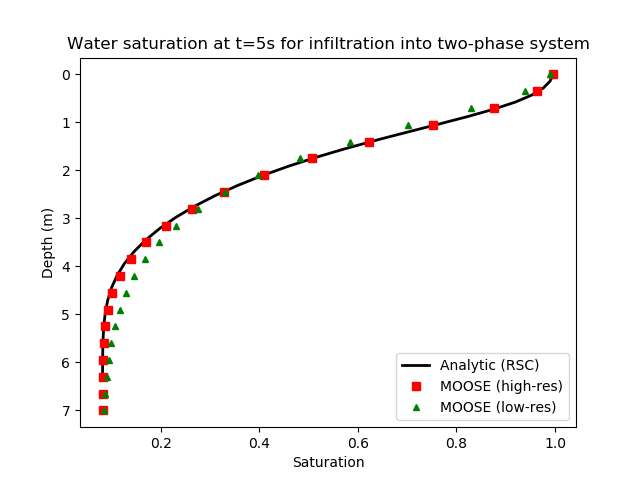
\includegraphics[width=16cm]{rsc.pdf}
\caption{Water saturation profile for $t=5$\,s in the
  Rogers-Stallybrass-Clements test.  The initial water saturation is
  0.08181, and water is injected at the top of this figure at a
  constant rate.  This forms a water front which displaces the oil.
  Black line: RSC's analytic solution.  Red squares: high-resolution
  MOOSE simulation.  Green triangles: lower resolution MOOSE simulation.}
\label{rsc.fig}
\end{center}
\end{figure}

\end{document}
